\documentclass[a4paper,10pt]{article}
\usepackage[utf8]{inputenc}
\usepackage{hyperref}
%opening
\title{Stockage de Données avec base de données MySQLd}
\author{Nicolas Vadkerti}
\usepackage{listings} % Required for inserting code snippets
\usepackage[usenames,dvipsnames]{color} % Required for specifying custom colors and referring to colors by name
\usepackage{graphicx}
\definecolor{DarkGreen}{rgb}{0.0,0.4,0.0} % Comment color
\definecolor{highlight}{RGB}{255,251,204} % Code highlight color

\lstdefinestyle{Style1}{ % Define a style for your code snippet, multiple definitions can be made if, for example, you wish to insert multiple code snippets using different programming languages into one document
language=Perl, % Detects keywords, comments, strings, functions, etc for the language specified
backgroundcolor=\color{highlight}, % Set the background color for the snippet - useful for highlighting
basicstyle=\footnotesize\ttfamily, % The default font size and style of the code
breakatwhitespace=false, % If true, only allows line breaks at white space
breaklines=true, % Automatic line breaking (prevents code from protruding outside the box)
captionpos=b, % Sets the caption position: b for bottom; t for top
commentstyle=\usefont{T1}{pcr}{m}{sl}\color{DarkGreen}, % Style of comments within the code - dark green courier font
deletekeywords={}, % If you want to delete any keywords from the current language separate them by commas
%escapeinside={\%}, % This allows you to escape to LaTeX using the character in the bracket
firstnumber=1, % Line numbers begin at line 1
frame=single, % Frame around the code box, value can be: none, leftline, topline, bottomline, lines, single, shadowbox
frameround=tttt, % Rounds the corners of the frame for the top left, top right, bottom left and bottom right positions
keywordstyle=\color{Blue}\bf, % Functions are bold and blue
morekeywords={}, % Add any functions no included by default here separated by commas
numbers=left, % Location of line numbers, can take the values of: none, left, right
numbersep=10pt, % Distance of line numbers from the code box
numberstyle=\tiny\color{Gray}, % Style used for line numbers
rulecolor=\color{black}, % Frame border color
showstringspaces=false, % Don't put marks in string spaces
showtabs=false, % Display tabs in the code as lines
stepnumber=5, % The step distance between line numbers, i.e. how often will lines be numbered
stringstyle=\color{Purple}, % Strings are purple
tabsize=2
}

\newcommand{\insertcode}[2]{\begin{itemize}\item[]\lstinputlisting[caption=#2,label=#1,style=Style1]{#1}\end{itemize}} 


% \insertcode{"Scripts/example.pl"}{Nena would be proud.} 

\begin{document}

\maketitle


\url{https://github.com/SlaynPool/CR_BDD/}

\section{Préparation (Installation des outils)}

 Suite  au passage à Debian 10, PHPmyAdmin n'est plus disponnible via les depots de APT, de ce fais, j'ai décidé d'utiliser Adminer, un gestionnaire de DATABASE equivalent, qui a la force d'etre qu'un seul fichier PHP donc très simple de déploiment.
 
 \insertcode{commande/1.txt}{Installation de Adminer }
\newpage
 \section{Mise en jambes}
 \subsection{Analyse de la base de test}
 \subsubsection{Analyser la nature de la base. Combien y a-t-il de tables dans la base?}
 La base a pour but de stocker des informations sur des pays, On peut voir qu'il ya trois tables dans la base :
 \insertcode{commande/2.txt}{SHOW TABLES}
 
  \subsubsection{Quelles sont les clefs primaire et secondaire des tables}
 Si l'on prend l'exemple de la table city :
 \insertcode{commande/3.txt}{SELECT * FROM city;}
 La pkey est  ID , et les clés secondaires sont : Name, CountryCode, District, Population.
 Cependant, les autres tables ont pour pkey : Code pour country et  CountryCode et language pour countrylanguage
 
 
 \subsection{Requetes de Base}
 \subsubsection{Donner la liste de toutes les villes françaises}
  \begin{figure}[h!]
\centering
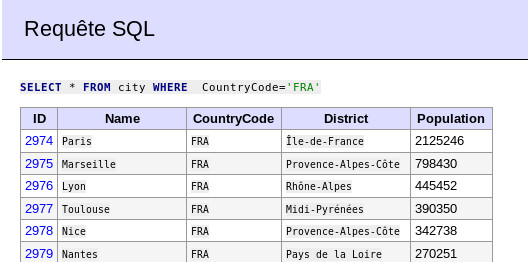
\includegraphics[scale=0.8]{ressource/1.jpg}
\caption{Notre requete SQL`}
\label{fig:paquet}
\end{figure}
\subsubsection{Récupérer la liste de toutes les capitales.}
Pour cette question j'ai trouvé deux solutions :

  \begin{figure}[h!]
\centering
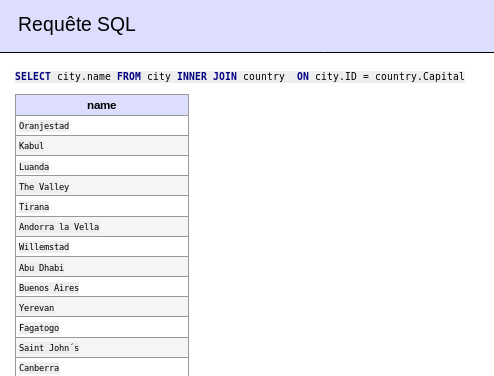
\includegraphics[scale=0.8]{ressource/2.jpg}
\caption{Solution 2}
\label{fig:paquet}
\end{figure}

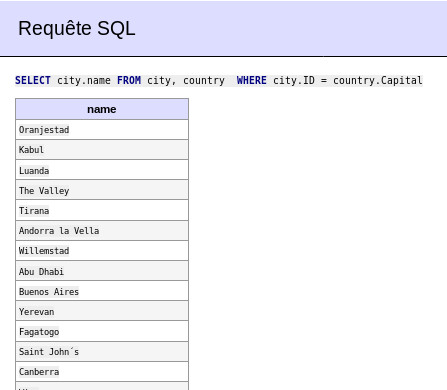
\includegraphics[scale=0.8]{ressource/3.jpg}

\newpage


\subsubsection{Combien y a-t-il de pays dans la base ? }
\insertcode{commande/5.txt}{count() }
\subsubsection{Donner les villes dont la population est supérieure à 1 million d’habitants. Combien de villescorrespondent à ce critère?}

\insertcode{commande/6.txt}{}

\end{document}

